\documentclass[11pt]{article}
\usepackage[T1]{fontenc}
\usepackage[utf8]{inputenc}
\usepackage{listings}
\usepackage{xcolor}
\usepackage{graphicx}
\definecolor{codegreen}{rgb}{0,0.6,0}
\definecolor{codegray}{rgb}{0.5,0.5,0.5}
\definecolor{codepurple}{rgb}{0.58,0,0.82}
\definecolor{backcolour}{rgb}{0.95,0.95,0.92}

\lstdefinestyle{mystyle}{
    backgroundcolor=\color{backcolour},   
    commentstyle=\color{codegreen},
    keywordstyle=\color{magenta},
    numberstyle=\tiny\color{codegray},
    stringstyle=\color{codepurple},
    basicstyle=\ttfamily\footnotesize,
    breakatwhitespace=false,         
    breaklines=true,                 
    captionpos=b,                    
    keepspaces=true,                 
    numbers=left,                    
    numbersep=5pt,                  
    showspaces=false,                
    showstringspaces=false,
    showtabs=false,                  
    tabsize=2
}

\lstset{style=mystyle}
\title{Algorytm genetyczny dla \\ problemu komiwojażera}
\author{Piotr Popis}
\date{Czerwiec 2020}
\begin{document}
\begin{titlepage}
\maketitle
\end{titlepage}
\section{Wprowadzenie}
\subsection{Problem komiwojażera( Traveling Salesman Problem)}
Jest jednym z najszerzej przebadanych problemów optymalizacji kombinatorycznej. Polega na zminimalizowaniu dystansu trasy Salesmana, gdzie trasa musi przechodzić przez zadane $n$ ( załóżmy, że ) $miast$ z jego listy, które powinien przejść dokładanie raz oraz znane są odległości pomiędzy miastami. Inaczej mówiąc szukamy minimalnego cyklu Hamiltona w pełnym grafie ważonym.\\
Problem możemy przedstawiać w różnych wariantach na przykład:
\begin{enumerate}
\item symetryczny sTSP
\item asymetryczny aTSP
\item wielokrotny mTSP
\item zgeneralizowany gTSP
\end{enumerate}
W symetrycznym przypadku odległość z miasta A do B jest taka sama jak odległość z B do A. W asymetrycznym odległości te mogą być różne ( $c_{ij} \neq c_{ji}$). W 3 przypadku wielokrotnym miasto może być odwiedzone więcej niż raz, a w przypadku zgeneralizowanym( uogólnionym) nie wszystkie miasta muszą być odwiedzone.
   Tego typu problemy powstają w różnych zastosowaniach ciekawymi przykładami są między innymi vehicle routing problem, printed circuit board punching sequence problems, wing nozzle design problem in air craft design. Należy do problemów NP- trudnych.
\subsection{Algorytm Genetyczny( Genetic Algorithm)}
\subsubsection{Opis}
Jest heurystyką, a mianowicie członkiem grupy algorytmów ewolucyjnych. Jest jedną z metod inteligencji obliczeniowej. Metodologia jest inspirowana efektywnością naturalnej selekcji w ewolucji biologicznej. W przeciwieństwie do innych metaheurystyk takich jak tabu serach czy simulated annealing nie generuje jednego rozwiązania, a grupę rozwiązań (generację). Bieżąca generacja nazywana jest populacją. Każdego członka bieżącej grupy nazywamy nieraz chromosomem. Do stworzenia nowej generacji używamy genotypów z poprzedniej generacji. Utworzenie nowego chromosomu, w zasadzie grupy chromosomów - generacji następuje zgodnie z różnymi operacjami.\\ Trzy najczęściej używane to: \begin{enumerate}
\item selekcja( selection),
\item krzyżowanie( crossover),
\item mutacja( mutation). 
\end{enumerate} 
Operacja selekcji pozwala wybrać odpowiednich osobników do nowych generacji. Wybiera zazwyczaj tych najlepszych, ale warto zostawić dla tych gorszych pewne prawdopodobieństwo wybrania w celu ucieczki z lokalnych optimum. Istnieje też możliwość rekombinacji czyli bezpośrednim przekazywaniu najlepszym osobników z populacji do nowej generacji w celu zachowania rozwiązań o bardzo wysokiej jakości. Krzyżowanie pozwala na wymieszanie genów wybranych w selekcji osobników. Mutacja natomiast polega na zazwyczaj losowym zmienieniu niektórych genów. Każda z powyższych operacji ma wiele efektywnych implementacji, które są zależne od problemu. Znaczy to tyle, że die da się jednoznacznie określić  najlepszej implementacji, tylko jedna jest bardziej dokładna obliczeniowo, inna znacznie szybsza.
\subsubsection{Schemat}
\centering
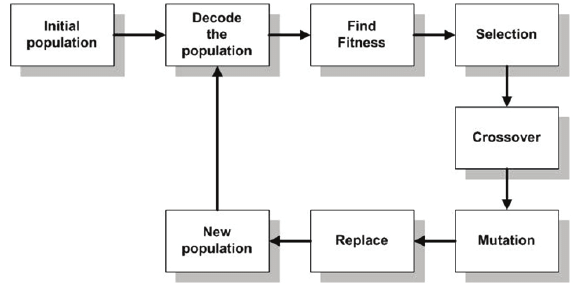
\includegraphics[scale=0.5]{ga_ex.png}
\flushleft
\subsection{Kilka wybranych implementacji powyższych operacji(pseudokod)}
\subsubsection{Selekcja}




\subsubsection{Krzyżowanie}
\paragraph{One-point crossover}-Zamiana suffixów dwóch osobników.
\begin{lstlisting}[language=Python ]
v,w - vectors ( paths)
c = randomint(1,l)
if c!=1:
	for i in (c,l):
		swap(vi,wi)
return v,w
\end{lstlisting}
\paragraph{Two-point crossover}Wymiana genów na zadanym przedziale c,d.
\begin{lstlisting}[language=Python]
v,w - vectors ( paths)
c,d = randomint(1,l),randomint(1,l)
if c>d:
	c,d=d,c
if c!=d:
	for i in (c,d-1):
		swap(vi,wi)
return v,w
\end{lstlisting}
\paragraph{Uniform crossover}Zamiana każdego genu z prawdopodobieństwem p.
\begin{lstlisting}[language=Python]
p - probab of swapping an index
v,w - vectors ( paths)
c,d = randomint(1,l),randomint(1,l)
for i in (1,l):
	if p>random.uniform(0,1):
		swap(vi,wi)
return v,w
\end{lstlisting}
\subsubsection{Mutacja}
\paragraph{Swap} Zamiana genów na pozycjach ( losowych i,j).
\begin{lstlisting}[language=Python]
i,j - random cities range(0,n)
return swap(path,i,j)
\end{lstlisting}
Teraz znając przykładowe implementacje operacji w algorytmie genetycznym głównie opierające się na permutacjach, możemy zacząć rozważania. Możemy postawić, że naszym celem jest znalezienie jak najbardziej optymalnego rozwiązania w jak najkrótszym czasie. Problemem stają się lokalne optima, których musimy pokonać odpowiednio dobierając operacje mutacji, krzyżowania oraz selekcji. Rozważmy kilka solucji problemu komiwojażera wykorzystując optymalny algorytm genetyczny.
\section{Różne strategie selekcji}
Jedną z operacji w algorytmie genetycznym jest selekcja. Służy do wybrania osobników, które następnie chcemy skrzyżować. Przy doborze rodziców musimy uważać, żeby nasze wybory nie doprowadziły do zamknięcia się na jeden genotyp
\subsection{Tournament Selection}
Bardzo popularną metodą jest selekcja turniejowa. Z większej populacji wybieramy x przedstawicieli losowo, wielkość x nazywamy rozmiarem turnieju. Binary Tournament zatem, to selekcja, w której do konkurencji wybieramy tylko 2 chromosomy. Następnie z wyodrębnionego zbioru wybieramy najlepszego. Takie podejście pozwala zachować różnorodność.\\
\centering
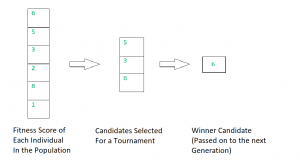
\includegraphics[scale=1.0]{ts.png}\\
\begin{lstlisting}[language=Python]
P - population
t- tounament size >0
best = random.choice(P)
for i from 2 to t:
	next = random.choice(P)
	if fitness(next)>fitness(Best)
		best=next
return best
\end{lstlisting}
\flushleft
\subsection{Proportional Roulette Wheel Selection}
Osobniki są wybierane z prawdopodobieństwem bezpośrednio proporcjonalnym do ich jakości (f -fitness value). Odpowiada to nieco kole ruletki.Koło możemy podzielić na segmenty odpowiadające proporcjom rodziców. Prawdopodobieństwo takie możemy wyznaczyć korzystając z wzoru $p_i=\frac{f_i}{\sum_{j=1}^nf_i}$. Główną zaletą jest to, że żaden z elementów populacji nie zostaje przekreślony. Ma też niestety swoje wady to znaczy, że jeśli populacja początkowa zawiera załóżmy, 2-3 silne genotypy, ale nie idealne, a pozostali członkowie populacji są bardzo słabi - zamknie się na tych dwóch najlepszych ( prawdopodobnie). Z drugiej strony słabe rozwiązania są szybko eliminowane. Jednak jeśli rozważamy problem minimalizacji to jest nieco uciążliwe rozwiązanie, bo musimy zaimplementować funkcje konwertującą funkcje minimalizującą do maksymalizującej. Wprowadza zatem lekkie zamieszanie.\\
\begin{center}
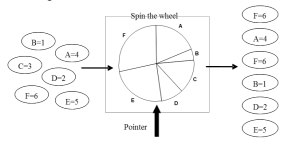
\includegraphics[scale=.8]{pwr.png}
\end{center} 
\begin{lstlisting}[language=Python]
do once per generation
	global p = [ind_1,...,ind_ps]
	global f = [fitness(pi) for pi in p]
	if f is all 0.0s:
		convert f to all 1.0s
	for i from 2 to l:
		fi = fi+ f_{i-1}
perform each time
	n = random(0,fl)
	for i from 2 to l:
		if  f_{i-1}<n<=fi:
			return pi
   return p1
\end{lstlisting}
\subsection{Rank-based Roulette Wheel Selection}
Prawdopodobieństwo wybrania chromosomu jest tutaj zależna od fitness value oraz jest relatywna do całej populacji. Najpierw osobnicy zostają posortowani zgodnie z ich jakością, a następnie wyliczane jest prawdopodobieństwo  na podstawie ich rankingu ,a nie bezpośrednim fitness. Potrzebujemy funkcji mapującej indeksy na posortowanej liście do listy jej prawdopodobieństw selekcji. Funkcja ta może, ale nie musi być liniowa. Bias może być regulowany przy użyciu nacisku wyboru SP dla liniowej np 2>SP>1. Pozycja zatem może być skalowana zgodnie z formułą:\\
$$Rank(Pos)=2-SP + (2.(SP-1).\frac{Pos-1}{n-1})$$ 
Można uniknąć skalowania, ale to może stać się bardziej kosztowne obliczeniowo z powodu sortowania. Takie podejście pozwala zablokować sytuację powodującą utknięcie w najlepszych chromosomach początkowych. Różnica pomiędzy kołami ruletki dla odpowiednio proporcjonalnej i rank-based selekcji.
\begin{center}
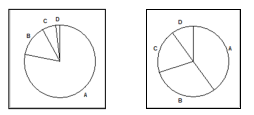
\includegraphics[scale=1.0]{rb.png}\\
Porównanie selekcji:
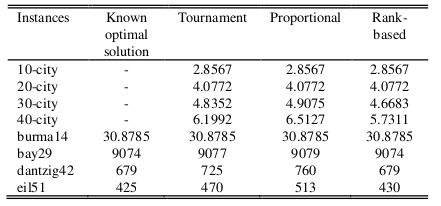
\includegraphics[scale=.7]{cs.png}

\end{center}
\section{Algorytm genetyczny bazujący na entropii}
\subsection{Opis}
Aby poradzić sobie z problemem lokalnego optimum Yasuhiro TSUJIMURA and Mitsuo GEN zaprezentowali rozwiązanie bazujące na entropii. Wykorzystali operację cycle crossover, swap mutation oraz selekcję - roulette wheel selection. Jak wiemy zwiększenie się ilości podobnych chromosomów w populacji może doprowadzić do utknięcia w lokalnym optimum. W EBGA mierzymy różnorodność chromosomów w każdej nowej generacji i ulepszamy populacje o małej różnorodności. Jak wyznaczyć zatem różnorodność? \\
\centering
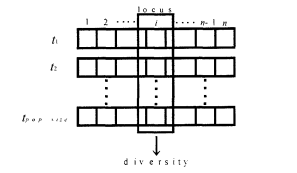
\includegraphics[scale=.7]{locus.png}\\
\flushleft
w tak ustawionych chromosomach przechodzimy po każdej kolumnie i sprawdzamy w niej różnorodność. Locus diversity $H_i$ i-tego locus możemy wyznaczyć ze wzoru:
$$H_i= \sum_{c \in C}pr_{ic}ln(pr_{ic})$$, gdzie
$pr_{ic}=\frac{na_{ic}}{population_{size}}$\\
C - zbiór miast\\
$ na_{ic}$ -ilość wystąpień miasta c na(index kolumny) locus i 
$ H_i $ osiąga maksymalną wartość $ln(population_{size})$, gdy każde miasto z C występuje jednolicie, a 0 gdy jedno z miast występuje znacznie częściej niż pozostałe. $H_i$ musimy oceniać na podstawie jakiejś stałej ( próg(ang. threshold)) w tym przypadku $ln2$.Jeśli próg jest większy lub równy $H_i$ to mamy niską różnorodność. Każde umiejscowienie porównujemy z progiem i jeśli jest większe od 
$\frac{n}{a}$ to zwięksamy podzielność. Parametr a to po prostu integer z przedziału [2,5]. Jak zwiększyć różnorodność? Korzystamy z procedury Med - Pop to znaczy, wybieramy $m=random(\frac{pop_{size}}{a},pop_{size}-1)$ chromosomów z populacji. W każdym wybranym chromosomie wymieniamy geny wzdłuż loca z innym mającym mniejszą różnorodność na locus niż próg.

\subsection{Podsumowanie}
\begin{enumerate}
\item Wygeneruj $pop_{size}$ chromosomów losowo.
\item Ewaluacja wyznacz jakość każdego chromosomu ( fitness) i oceń, który jest najlepszy $eval(t_k) = \frac{1}{\sum_{i=1}^{n}d(c_i,c_{i+1})+d(c_n,c_1)}$
\item Krzyżowanie CX cycle crossover na wybranych chromosomach z prawdopodobieństwem pr
\item Mutacja zamiana miast z prawdopodobieństwem pm
\item selekcja wybierz $pop_{size}$ chromosomów korzystając z roulette wheel selection.
\item Ulepsz różnorodność populacji korzystając z procedury med-pop.
\end{enumerate}
\centering
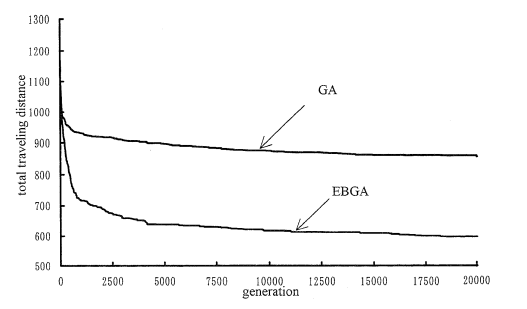
\includegraphics[scale=0.5]{ebga_ga.png}\\
\flushleft
Jak widać EBGA znajduje dużo lepsze rozwiązania niż GA.

\end{document}